%!TEX TS-program = xelatex
%!TEX encoding = UTF-8 Unicode

\documentclass[oneside,School=Harvard]{Dissertate}

\geometry{
    a4paper,
    margin=1in,
    %showframe=true,
}

\usepackage[export]{adjustbox}
\usepackage{color}
\usepackage{csquotes}
\usepackage{excludeonly}
\usepackage{fancyvrb}
\usepackage{imakeidx}
\usepackage{listings}
\usepackage{microtype}
\usepackage{multicol}
\usepackage{pdfpages}
\usepackage{textcomp}
\usepackage[color=yellow]{todonotes}

\usepackage[
    labelfont={sc,scriptsize},
    textfont={rm,scriptsize},
    singlelinecheck=off,
]{caption}

%\usepackage[margincaption,outercaption,raggedright]{sidecap}
%\sidecaptionvpos{figure}{t} 
%\sidecaptionvpos{table}{t}

\usepackage{sidenotes}

\newenvironment{markdown}{
    \VerbatimEnvironment
    \begin{VerbatimOut}{tmp/tmp.markdown}%
}{  
    \end{VerbatimOut}
    \immediate\write18{pandoc tmp/tmp.markdown -t latex -o tmp/tmp.tex}
    \input{tmp/tmp.tex}
}

\definecolor{bluekeywords}{rgb}{0.13,0.13,1}
\definecolor{greencomments}{rgb}{0,0.5,0}
\definecolor{redstrings}{rgb}{0.9,0,0}
\definecolor{grey}{rgb}{0.5,0.5,0.5}
\definecolor{lightgrey}{rgb}{0.75,0.75,0.75}

\lstset{
    basicstyle=\scriptsize\ttfamily,
    breakatwhitespace=false,
    breaklines=false,
    commentstyle=\color{greencomments},
    escapeinside={(*@}{@*)},
    frame=l,
    framerule=1.5pt,
    framesep=6pt,
    keywordstyle=\color{bluekeywords}\bfseries,
    language=Python,
    showspaces=false,
    showstringspaces=false,
    showtabs=false,
    stringstyle=\color{redstrings},
    upquote=true,
}

\lstdefinestyle{beep}{
    language=[LaTeX]TeX,
}

\includeonly{
%    source/chapters/introduction,
%    source/chapters/a-model-of-notation,
    source/chapters/time-tools,
    source/chapters/a-model-of-composition,
%    source/chapters/practicalities,
%    source/chapters/conclusion,
}

%\excludeonly{
%    source/chapters/score-aurora,
%    source/chapters/score-plague-water,
%    source/chapters/score-zaira,
%    source/chapters/score-armilla,
%    source/chapters/score-ersilia,
%}

\makeindex[columns=3, title=Index, intoc]

\begin{document}

\frontmatter
\pagenumbering{roman}
% Some details about the dissertation.
\title{How to cook an egg}
\author{Josiah Wolf Oberholtzer}
\advisor{Hans Tutschku \& Chaya Czernowin}

% ... about the degree.
\degree{Doctor of Philosophy}
\field{Music Composition}
\degreeyear{2015}
\degreemonth{May}
\department{Music}

% ... about the candidate's previous degrees.
\pdOneName{B.Mus.}
\pdOneSchool{Oberlin Conservatory}
\pdOneYear{2006}

%\pdTwoName{M.A.}
%\pdTwoSchool{Monster's Univeristy}
%\pdTwoYear{2021}
\maketitle
%\copyrightpage
%\abstractpage
\tableofcontents
%\listoffigures
%\dedicationpage
%\acknowledgments

\mainmatter
\doublespacing
\cleardoublepage
\pagenumbering{arabic}
\setcounter{page}{1}
\setcounter{chapter}{-1}

%%%%%%%%%%%%%%%%%%%%%%%%%%%%%%%%%%%%%%%%%%%%%%%%%%%%%%%%%%%%%%%%%%%%%%%%%%%%%%%
%%%%%%%%%%%%%%%%%%%%%%%%%%%%%%%%%%%%%%%%%%%%%%%%%%%%%%%%%%%%%%%%%%%%%%%%%%%%%%%
\chapter{Introduction}
\label{chap:introduction}
%%%%%%%%%%%%%%%%%%%%%%%%%%%%%%%%%%%%%%%%%%%%%%%%%%%%%%%%%%%%%%%%%%%%%%%%%%%%%%%
%%%%%%%%%%%%%%%%%%%%%%%%%%%%%%%%%%%%%%%%%%%%%%%%%%%%%%%%%%%%%%%%%%%%%%%%%%%%%%%

\begin{figure}
\begin{centering}
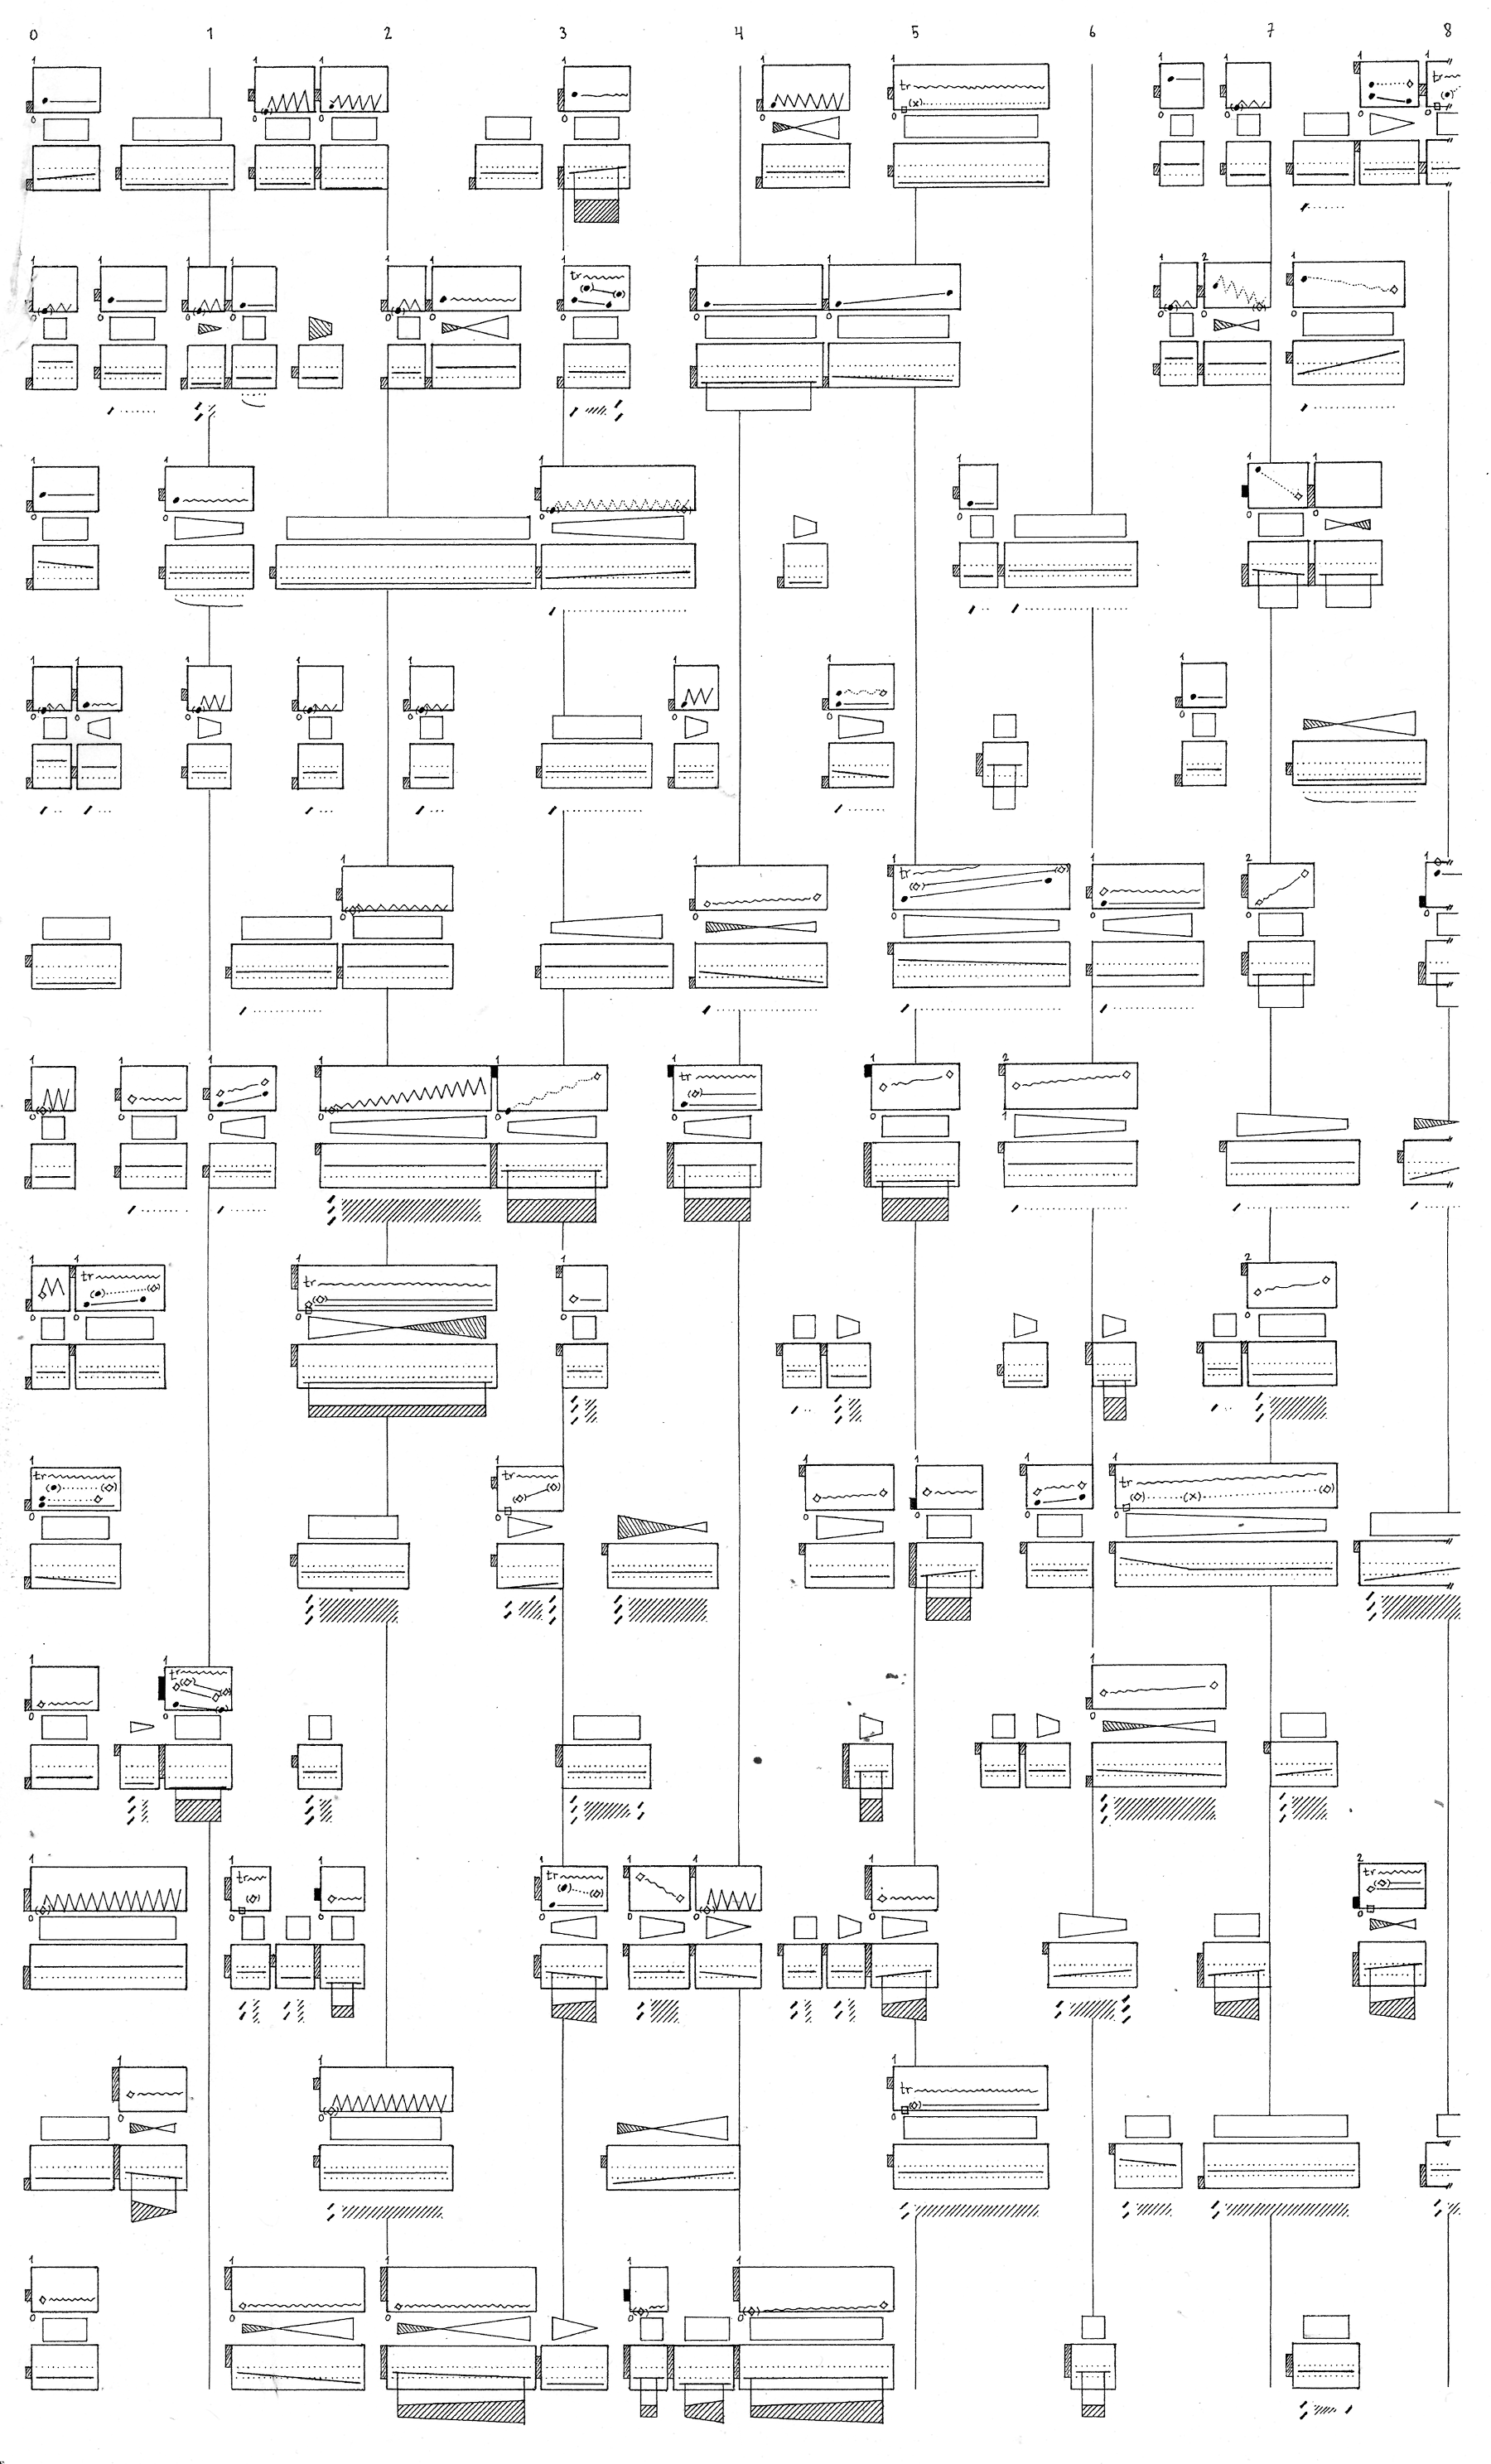
\includegraphics[
    page=1,
    width=\textwidth,
    height=0.9\textheight,
    keepaspectratio,
]{assets/dissertation-score-mbrsi.pdf}
\caption{The first page of \emph{mbrsi} (2006), an unfinished tablature score
for one to twelve string performers. This represents an early attempt of mine
at computationally modeling massed performers with timespans to create an
evolving \enquote{granular} texture. The instructions for the score were
created through a variety of Max/MSP patches which painstakingly converted
noise functions into text files which I then collated into spreadsheets. The
score itself was drawn by hand on size A1 graph paper with Rapidographs.
I completed seventeen of the intended fifty-three pages before stopping for the
sake of my wrists and due a general lack of faith in the project. While still
incomplete, the concerns that motivated this score remain with me.}
\end{centering} \end{figure}

\begin{figure}
\begin{centering}
\noindent\includegraphics[
    page=1,
    width=\textwidth,
]{assets/dissertation-score-mbrsi-lh.pdf}
\caption{Page one of fifty-three from a spreadsheet containing fingering
instructions for six of the twelve string performers in \emph{mbrsi} (2006).}
\end{centering}
\end{figure}

\begin{figure}
\begin{centering}
\noindent\includegraphics[
    clip=true,
    trim=0in 0.125in 0in 0in,
    page=1,
    width=\textwidth,
]{assets/dissertation-score-mbrsi-rh.pdf}
\caption{Page one of fifty-three from a spreadsheet containing bowing
instructions for six of the twelve string performers in \emph{mbrsi} (2006).}
\end{centering}
\end{figure}

\begin{markdown}

# What is this?

Laying out the terms.

This is an analysis of a model of composition, implemented computationally.

This is not an analysis of any works, although works are included.

This is not a survey of techniques used by composers working in
computer-assisted composition, but the work of one composer implementing for
the specifics of his own process. This work may well be applicable to others in
many ways, but I do not claim universality.

Provide a description of formalized score control.

Mention Abjad, Python, LilyPond and LaTeX very briefly. Drop names as
appropriate.

My aim is to provide a sufficiently detailed explanation of the theory behind
this work as well as my specific implementation that those who read
this would be able to consult the source to each of the three Invisible Cities
scores included in the appendices and make some (or a lot of) sense of them.

It is then, more of a tutorial than anything else, presented in order to
explain the architectural decisions, implementations and implications behind a
system designed to assist in the composition of music.

# Background

Mention Trevor Wishart's \emph{On Sonic Art} with regard to textural variation,
and Curtis Roads' \emph{Microsound} for granular techniques.

Both historical and personal.

Provide wider discussion of Abjad, Python, LilyPond and LaTeX.

Differentiate from Max, PWGL, OM.

# Overview of the dissertation

This dissertation consists of six chapters of prose -- including this chapter
--, followed by five chapters each presenting a score, and four extensive
appendices comprising complete code listings for the implementations of the
scores and of Consort. Please consult the source for Abjad directly, as it is
far too large to include here.

The first six chapters 

Chapter 2 presents an overview of Abjad, detailing its structure and usage in
the creation of scores.

Chapter 3 expands on chapter 2, discussing various models of musical time in
detail, and introducing many of tools and techniques employed in Consort to
create large-scale musical works.

Chapter 4 analyzes the mechanisms implemented in Consort to specify the
structure of scores at a high level and to interpret those specifications in
order to produce notation.

Chapter 5 discusses practical concerns surrounding the composition of scores in
software including project layout, typesetting workflows, version control and
testing.

Chapter 6, the conclusion to the prose portion of the dissertation, summarizes
the previously presented research, and suggests implications and future work.

The remaining chapters consist of five scores, all composed computationally
with Python and LilyPond.

Chapter 7, Aurora/Mbrsi

- my first formal research into composition with timespans

Chapter 8, Plague Water

- my first attempt at composing scores in segments, implemented with the
precursor to Consort

Chapters 9, 10 and 11 present a set of three pieces, Invisible Cities (i):
Zaira, Invisible Cities (ii): Armilla and Invisible Cities (iii): Ersilia, all
implemented via Consort.

The appendices contain the source to all classes and functions implemented in
Consort, as well as the source to all material and segment definitions, as well
as any LilyPond stylesheets, for the three Invisible Cities scores.

\end{markdown}
%%%%%%%%%%%%%%%%%%%%%%%%%%%%%%%%%%%%%%%%%%%%%%%%%%%%%%%%%%%%%%%%%%%%%%%%%%%%%%%
%%%%%%%%%%%%%%%%%%%%%%%%%%%%%%%%%%%%%%%%%%%%%%%%%%%%%%%%%%%%%%%%%%%%%%%%%%%%%%%
\chapter{\emph{Abjad}: a model of notation}
\label{chap:a-model-of-notation}
%%%%%%%%%%%%%%%%%%%%%%%%%%%%%%%%%%%%%%%%%%%%%%%%%%%%%%%%%%%%%%%%%%%%%%%%%%%%%%%
%%%%%%%%%%%%%%%%%%%%%%%%%%%%%%%%%%%%%%%%%%%%%%%%%%%%%%%%%%%%%%%%%%%%%%%%%%%%%%%

\begin{comment}
<abjad>[hide=true]
import collections
import consort
</abjad>
\end{comment}

Abjad models notation.

%%%%%%%%%%%%%%%%%%%%%%%%%%%%%%%%%%%%%%%%%%%%%%%%%%%%%%%%%%%%%%%%%%%%%%%%%%%%%%%
\section{The illustration protocol}
%%%%%%%%%%%%%%%%%%%%%%%%%%%%%%%%%%%%%%%%%%%%%%%%%%%%%%%%%%%%%%%%%%%%%%%%%%%%%%%

foo

\begin{markdown}
-   print()
-   repr() and __repr__()
-   str() and __str__()
-   format() and __format__()
-   show() and __illustrate__()
-   graph() and __graph__()
\end{markdown}

%%%%%%%%%%%%%%%%%%%%%%%%%%%%%%%%%%%%%%%%%%%%%%%%%%%%%%%%%%%%%%%%%%%%%%%%%%%%%%%
\section{Components, leaves \& containers}
%%%%%%%%%%%%%%%%%%%%%%%%%%%%%%%%%%%%%%%%%%%%%%%%%%%%%%%%%%%%%%%%%%%%%%%%%%%%%%%

\begin{markdown}
-   The score tree
-   Component
-   Count-time components
-   Non-count-time components
-   One, and only one, parent per component. They *cannot* be in more than one
    container. This is both confusing, and liable to cause reference problems.
\end{markdown}

\subsection{Leaves}

\begin{markdown}
-   Leaf
-   These are components which do not contain other components.
-   Note
-   Rest
-   Chord
-   NoteHead
\end{markdown}

\subsection{Containers}

\begin{markdown}
-   Container
-   LilyPond and { }
-   Measure
-   LilyPond has no explicit measures
-   Tuplet and FixedDurationTuplet
\end{markdown}

\subsection{Contexts}

\begin{markdown}
-   Context
-   Contexts are containers, but not *count-time*
-   Voice
-   Staff
-   StaffGroup
-   Score
\end{markdown}

\subsection{Inspection}

\begin{markdown}
-   inspect_()
-   not *inspect()*, as that would cause a name conflict with Python's inspect
    module
-   inspect(...).get_parentage()
\end{markdown}

\begin{comment}
<abjad>
upper_staff = Staff(name='Upper Staff')
lower_staff = Staff(name='Lower Staff')
staff_group = StaffGroup([upper_staff, lower_staff])
score = Score([staff_group])
</abjad>
\end{comment}

%%%%%%%%%%%%%%%%%%%%%%%%%%%%%%%%%%%%%%%%%%%%%%%%%%%%%%%%%%%%%%%%%%%%%%%%%%%%%%%
\section{Durations, offsets \& timespans}
%%%%%%%%%%%%%%%%%%%%%%%%%%%%%%%%%%%%%%%%%%%%%%%%%%%%%%%%%%%%%%%%%%%%%%%%%%%%%%%

foo

\subsection{Operations on durations}

\begin{comment}
<abjad>
Duration(1, 2) + Duration(3, 4)
Offset(1, 2) + Duration(3, 4)
Offset(7, 8) - Offset(1, 12)
</abjad>
\end{comment}

\subsection{Inspecting durations}

\begin{markdown}
-   inspect_(...).get_duration()
-   inspect_(...).get_timespan()
-   in_seconds=True
\end{markdown}

%%%%%%%%%%%%%%%%%%%%%%%%%%%%%%%%%%%%%%%%%%%%%%%%%%%%%%%%%%%%%%%%%%%%%%%%%%%%%%%
\section{Pitches, pitch-classes, intervals and operators}
%%%%%%%%%%%%%%%%%%%%%%%%%%%%%%%%%%%%%%%%%%%%%%%%%%%%%%%%%%%%%%%%%%%%%%%%%%%%%%%

foo

\subsection{Pitch representations}

\begin{markdown}
- NamedPitch
- NumberedPitch
- NamedPitchClass
- NumberedPitchClass
\end{markdown}

\begin{markdown}
- NamedInterval
- NumberedInterval
- NamedIntervalClass
- NumberedIntervalClass
- NamedInversionEquivalentIntervalClass
- NumberedInversionEquivalentIntervalClass
\end{markdown}

\subsection{Pitch collections}

\begin{markdown}
- Set, Segment, Vector
- Pitch, PitchClass, Interval, IntervalClass
\end{markdown}

\begin{markdown}
- PitchSegment
- PitchClassSegment
\end{markdown}

\subsection{Pitch operators}

\begin{comment}
<abjad>
pitch_segment = pitchtools.PitchSegment("c' ef' b' bf' f' e' b a")
show(pitch_segment)
</abjad>
\end{comment}

\begin{comment}
<abjad>
transposition = pitchtools.Transposition(1)
show(transposition(pitch_segment))
</abjad>
\end{comment}

\begin{comment}
<abjad>
inversion = pitchtools.Inversion()
show(inversion(pitch_segment))
inversion_with_axis = pitchtools.Inversion(axis=NamedPitch("d'"))
show(inversion_with_axis(pitch_segment))
</abjad>
\end{comment}

\begin{comment}
<abjad>
retrogression = pitchtools.Retrogression()
show(retrogression(pitch_segment))
</abjad>
\end{comment}

\begin{comment}
<abjad>
untransposing_rotation = pitchtools.Rotation(-1, transpose=False)
show(untransposing_rotation(pitch_segment))
transposing_rotation = pitchtools.Rotation(-1, transpose=True)
show(transposing_rotation(pitch_segment))
</abjad>
\end{comment}

\begin{comment}
<abjad>
multiplication = pitchtools.Multiplication(3)
show(multiplication(pitch_segment))
</abjad>
\end{comment}

\begin{comment}
<abjad>
pitch_operation = pitchtools.PitchOperation(
    operators=(
        pitchtools.Rotation(1),
        pitchtools.Transposition(2),
        ),
    )
show(pitch_operation(pitch_segment))
</abjad>
\end{comment}

\subsection{Other pitch modeling concepts}

\begin{markdown}
-   Accidental
-   Octave
-   PitchRange
-   StaffPosition
\end{markdown}

\subsection{Inspecting leaf pitches}

\begin{markdown}
-   Note("c'4").written_pitch
-   Note("c'4").note_head.written_pitch
-   Chord("<c' e' g'>4").written_pitches
-   inspect_(note).get_sounding_pitch()
-   inspect_(note).get_sounding_pitches()
\end{markdown}

%%%%%%%%%%%%%%%%%%%%%%%%%%%%%%%%%%%%%%%%%%%%%%%%%%%%%%%%%%%%%%%%%%%%%%%%%%%%%%%
\section{Indicators}
%%%%%%%%%%%%%%%%%%%%%%%%%%%%%%%%%%%%%%%%%%%%%%%%%%%%%%%%%%%%%%%%%%%%%%%%%%%%%%%

\subsection{Attachment}

\begin{markdown}
-   attach(x, y, scope=..., is_annotation=..., name=...)
\end{markdown}

\subsection{Tour of indicators}

\begin{markdown}
-   Articulation
-   BarLine
-   Clef
-   Dynamic
-   KeySignature
-   Markup
-   Tempo
-   TimeSignature
\end{markdown}

\subsection{Context scoping}

\begin{markdown}
-   What is scope?
-   Default scope
-   Explicit scope
\end{markdown}

\subsection{Non-formatting annotations}

\begin{markdown}
-   Annotation
-   Idiomatic indicators, used by other processes:
    -   BowContactPoint
    -   IsAtSoundingPitch
    -   IsUnpitched
    -   StringContactPoint
    -   StringTuning
    -   etc.
-   attach(x, y, is_annotation=True)
\end{markdown}

%%%%%%%%%%%%%%%%%%%%%%%%%%%%%%%%%%%%%%%%%%%%%%%%%%%%%%%%%%%%%%%%%%%%%%%%%%%%%%%
\section{Spanners}
%%%%%%%%%%%%%%%%%%%%%%%%%%%%%%%%%%%%%%%%%%%%%%%%%%%%%%%%%%%%%%%%%%%%%%%%%%%%%%%

\begin{markdown}
-   graph cyclicity
-   logical voices
\end{markdown}

\subsection{Tour of spanners}

\begin{markdown}
-   Beam
-   Glissando
-   Hairpin
-   Slur
-   Trill
-   Tie
\end{markdown}

\subsection{LilyPond format bundles}

foo

\subsection{Complex conditional formatting}

foo

\subsection{Complex indicators}

\begin{markdown}
-   KeyCluster
\end{markdown}

%%%%%%%%%%%%%%%%%%%%%%%%%%%%%%%%%%%%%%%%%%%%%%%%%%%%%%%%%%%%%%%%%%%%%%%%%%%%%%%
\section{Score iteration, selections \& selectors}
%%%%%%%%%%%%%%%%%%%%%%%%%%%%%%%%%%%%%%%%%%%%%%%%%%%%%%%%%%%%%%%%%%%%%%%%%%%%%%%

foo

\subsection{Indexing}
\label{ssec:indexing}

\begin{markdown}
-   By name
-   By index
-   By slice
\end{markdown}

\subsection{Selection}
\label{ssec:selection}

\begin{markdown}
-   select()
-   Selection class
-   Container.select_leaves()
    -   allow_discontiguous_leaves=True
-   inspect_(...).get_logical_tie()
-   LogicalTie
    -   head
    -   tail
    -   timespan
    -   trivial logical ties
\end{markdown}

\subsection{Iteration}
\label{ssec:iteration}

\begin{markdown}
-   By __iter__()
-   By iterate(...)by_...()
    -   by_class()
    -   by_logical_tie()
    -   by_run()
    -   by_timeline()
    -   by_vertical_moment()
    -   depth_first()
\end{markdown}

\subsection{Selectors}
\label{ssec:selectors}

\begin{markdown}
-   Demonstrate a gallery of selectors.
    -   by duration
    -   by leaves
    -   by length
    -   by logical tie
    -   by counts (with negative counts too)
\end{markdown}

%%%%%%%%%%%%%%%%%%%%%%%%%%%%%%%%%%%%%%%%%%%%%%%%%%%%%%%%%%%%%%%%%%%%%%%%%%%%%%%
\section{Notation factories}
%%%%%%%%%%%%%%%%%%%%%%%%%%%%%%%%%%%%%%%%%%%%%%%%%%%%%%%%%%%%%%%%%%%%%%%%%%%%%%%

foo

\subsection{Rhythm makers}

foo

\subsection{Score templates}
\label{ssec:score-templates}

\begin{markdown}
-   Simplify score creation process
\end{markdown}

\subsection{Parsers}

\begin{markdown}
-   LilyPond parser
-   PLY
-   SchemeParser
-   RhythmTreeParser
-   ReducedLyParser
\end{markdown}
%%%%%%%%%%%%%%%%%%%%%%%%%%%%%%%%%%%%%%%%%%%%%%%%%%%%%%%%%%%%%%%%%%%%%%%%%%%%%%%
\chapter{Tools for modeling time, rhythm and meter}
%%%%%%%%%%%%%%%%%%%%%%%%%%%%%%%%%%%%%%%%%%%%%%%%%%%%%%%%%%%%%%%%%%%%%%%%%%%%%%%

\begin{comment}
<abjad>[hide=true]
import consort
</abjad>
\end{comment}

Consort's implementation of a model of composition relies on a number of
different but interrelated models of musical time. A thorough discussion of
these time models here will clarify the analysis of Consort's implementation in
the following chapters.

Dichotomies: outside and inside the score hierarchy, with or without regard to
notation, "coarse" versus "fine" or "phrase" versus "event", vertical or
horizontal, metered and unmetered, potentially simultaneous or strictly
contiguous.

Timespans provide a coarse model of musical time, both in and outside of score
hierarchy.

Notated rhythm provides a fine model of musical time, from within score
hierarchy.

Meter coordinates time and rhythm vertically across score hierarchy, and
bridges the coarse and fine stages of rhythmic interpretation.

Meter is generated as a by-product of phrase-level composition. It is not
specified by-hand during composition. This is not out of any desire to valorize
automaticism, but simply because lacking any other compelling reason to
generate a series of meters I felt the best way for myself would be to have
those meters derive from some sort of pre-existent structure in my
compositional process.

A discussion of these time models and their implications will clarify a later
analysis of the implementation of Consort's score interpretation
stage.

%%%%%%%%%%%%%%%%%%%%%%%%%%%%%%%%%%%%%%%%%%%%%%%%%%%%%%%%%%%%%%%%%%%%%%%%%%%%%%%
\section{Timespans}
%%%%%%%%%%%%%%%%%%%%%%%%%%%%%%%%%%%%%%%%%%%%%%%%%%%%%%%%%%%%%%%%%%%%%%%%%%%%%%%

A timespan is simply a start offset paired with a stop offset as a closed/open
interval\footnote{Add a discussion of the mathematical definition of closed and
open intervals here.}. Timespans represent an interval of time, of duration 0
or greater, positioned somewhere along an arbitrary timeline. Every durated
object in a score \emph{has} a timespan -- including the score itself, but
timespans exist -- by definition -- without regard for any specific score, in
whole or part.

Abjad models timespans as the class \texttt{timespantools.Timespan}.

\begin{comment}
<abjad>
timespan = timespantools.Timespan(
    start_offset=Offset(1, 4),
    stop_offset=Offset(3, 2),
    )
</abjad>
\end{comment}

\subsection{Inspecting timespans}

\begin{comment}
<abjad>
timespan.start_offset
timespan.stop_offset
timespan.duration
</abjad>
\end{comment}

\begin{comment}
<abjad>
malformed_timespan = timespantools.Timespan(0, 0)
malformed_timespan.is_well_formed
</abjad>
\end{comment}

\begin{comment}
<abjad>
templated_timespan = new(timespan, stop_offset=(5, 16))
print(format(templated_timespan))
</abjad>
\end{comment}

\begin{comment}
<abjad>
annotated_timespan = timespantools.AnnotatedTimespan(
    start_offset=(1, 8),
    stop_offset=(7, 8),
    annotation='Any arbitrary object can act as an annotation.'
    )
annotated_timespan.annotation
</abjad>
\end{comment}

\subsection{Time relations}

- time relations: intersection, congruency etc.

\begin{comment}
<abjad>
timespan_1 = timespantools.Timespan(0, 10)
timespan_2 = timespantools.Timespan(5, 15)
timespan_3 = timespantools.Timespan(10, 15)
</abjad>
\end{comment}

\begin{comment}
<abjad>
timespan_1.intersects_timespan(timespan_2)
timespan_1.intersects_timespan(timespan_3)
timespan_2.intersects_timespan(timespan_1)
timespan_2.intersects_timespan(timespan_3)
timespan_3.intersects_timespan(timespan_1)
timespan_3.intersects_timespan(timespan_2)
</abjad>
\end{comment}

\begin{comment}
<abjad>
timespan_1.is_congruent_to_timespan(timespan_2)
timespan_1.is_congruent_to_timespan(timespan_1)
</abjad>
\end{comment}

\begin{comment}
<abjad>
timespan_1.is_tangent_to_timespan(timespan_2)
timespan_1.is_tangent_to_timespan(timespan_3)
</abjad>
\end{comment}

\subsection{Operations on timespans}

Consider the following three timespans again.

\begin{comment}
<abjad>
timespan_1 = timespantools.Timespan(0, 10)
timespan_2 = timespantools.Timespan(5, 15)
timespan_3 = timespantools.Timespan(10, 15)
</abjad>
\end{comment}

The logical AND of any two timespans can be computed.

\begin{comment}
<abjad>
timespan_1 & timespan_2
timespan_1 & timespan_3
timespan_2 & timespan_3
</abjad>
\end{comment}

The logical OR of any two timespans can be computed.

\begin{comment}
<abjad>
timespan_1 | timespan_2
timespan_1 | timespan_3
timespan_2 | timespan_3
</abjad>
\end{comment}

Timespan subtraction is another crucial operation.

\begin{comment}
<abjad>
timespan_1 = timespantools.Timespan(0, 15)
timespan_2 = timespantools.Timespan(5, 10)
timespan_3 = timespantools.Timespan(10, 20)
</abjad>
\end{comment}

\begin{comment}
<abjad>
print(format(timespan_1 - timespan_1))
print(format(timespan_1 - timespan_2))
print(format(timespan_1 - timespan_3))
print(format(timespan_2 - timespan_1))
print(format(timespan_2 - timespan_2))
print(format(timespan_2 - timespan_3))
print(format(timespan_3 - timespan_1))
print(format(timespan_3 - timespan_2))
print(format(timespan_3 - timespan_3))
</abjad>
\end{comment}

%%%%%%%%%%%%%%%%%%%%%%%%%%%%%%%%%%%%%%%%%%%%%%%%%%%%%%%%%%%%%%%%%%%%%%%%%%%%%%%
\section{Timespan inventories}
%%%%%%%%%%%%%%%%%%%%%%%%%%%%%%%%%%%%%%%%%%%%%%%%%%%%%%%%%%%%%%%%%%%%%%%%%%%%%%%

Timespans can be aggregated together in an instance of the TimespanInventory
class. In addition to the protocol defined for ordered collections, timespan
inventories provide a variety of other methods and properties for working
specifically with timespans.

\begin{comment}
<abjad>
timespan_inventory = timespantools.TimespanInventory()
timespan_inventory.append(timespantools.Timespan(0, 16))
timespan_inventory.append(timespantools.Timespan(5, 12))
timespan_inventory.append(timespantools.Timespan(-2, 8))
timespan_inventory.append(timespantools.Timespan(15, 20))
print(format(timespan_inventory))
</abjad>
\end{comment}

\subsection{Inspecting timespan inventories}

\begin{comment}
<abjad>
len(timespan_inventory)
timespan_inventory[1]
for timespan in timespan_inventory:
    timespan
    
</abjad>
\end{comment}

\begin{comment}
<abjad>
timespan_inventory.start_offset
timespan_inventory.stop_offset
timespan_inventory.duration
timespan_inventory.timespan
timespan_inventory.all_are_contiguous
timespan_inventory.all_are_nonoverlapping
timespan_inventory.all_are_well_formed
</abjad>
\end{comment}

\subsection{Unioning, differencing and splitting}

\begin{comment}
<abjad>
timespan_inventory = timespantools.TimespanInventory([
    timespantools.Timespan(0, 16),
    timespantools.Timespan(5, 12),
    timespantools.Timespan(-2, 8),
    ])
timespan = timespantools.Timespan(5, 10)
result = timespan_inventory & timespan
print(format(timespan_inventory))
</abjad>
\end{comment}

\begin{comment}
<abjad>
timespan_inventory = timespantools.TimespanInventory([
    timespantools.Timespan(0, 16),
    timespantools.Timespan(5, 12),
    timespantools.Timespan(-2, 8),
    ])
timespan = timespantools.Timespan(5, 10)
result = timespan_inventory - timespan
print(format(timespan_inventory))
</abjad>
\end{comment}

\begin{comment}
<abjad>
timespan_inventory = timespantools.TimespanInventory([
    timespantools.Timespan(0, 3),
    timespantools.Timespan(3, 6),
    timespantools.Timespan(6, 10),
    ])
left, right = timespan_inventory.split_at_offset(4)
print(format(left))
print(format(right))
</abjad>
\end{comment}

\begin{comment}
Timespan.split_at_offsets()
\end{comment}

\subsection{Timewise partitioning}

\begin{comment}
<abjad>
timespan_inventory = timespantools.TimespanInventory([
    timespantools.Timespan(0, 10),
    timespantools.Timespan(5, 15),
    timespantools.Timespan(15, 20),
    timespantools.Timespan(25, 30),
    ])
</abjad>
\end{comment}

\begin{comment}
<abjad>
for inventory in timespan_inventory.partition():
    print(format(inventory))

</abjad>
\end{comment}

\begin{comment}
<abjad>
for inventory in timespan_inventory.partition(include_tangent_timespans=True):
    print(format(inventory))

</abjad>
\end{comment}

\subsection{Other timespan inventory operations}

\begin{comment}
TimespanInventory.clip_timespan_durations
TimespanInventory.count_offsets()
TimespanInventory.explode()
TimespanInventory.round_offsets()
\end{comment}

\subsection{Optimized timespan inventories}

Consort provides its own timespan collection class -- the TimespanCollection.
This class stores timespans internally not as a list, but in a balanced
\emph{interval tree}\footnote{An interval tree is an augmented self-balancing
binary tree which stores both start offsets as well as stop offsets.}
datastructure which guarantees sorting and allows for highly optimized lookups
of timespans intersecting specific offsets. This class is used at crucial
points during Consort's interpretation stage simply for purposes of speed, and
should be considered an implementation detail. With work, its internal
datastructure will eventually be merged into Abjad's TimespanInventory.

%%%%%%%%%%%%%%%%%%%%%%%%%%%%%%%%%%%%%%%%%%%%%%%%%%%%%%%%%%%%%%%%%%%%%%%%%%%%%%%
\section{Annotated timespans in \emph{Consort}}
%%%%%%%%%%%%%%%%%%%%%%%%%%%%%%%%%%%%%%%%%%%%%%%%%%%%%%%%%%%%%%%%%%%%%%%%%%%%%%%

We need to discuss the products of timespan makers before we can discuss
timespan makers themselves.

\subsection{Payloaded timespans}

- layer

- voice name

\subsection{\emph{Performed} timespans}

\begin{comment}
<abjad>
performed_timespan = consort.PerformedTimespan(
    layer=1,
    minimum_duration=Duration(1, 8),
    music_specifier=consort.MusicSpecifier(),
    start_offset=Offset(1, 4),
    stop_offset=Offset(2, 1),
    voice_name='Violin 1 LH Voice',
    )
</abjad>
\end{comment}

- forbid fusing

- forbid splitting

- minimum duration

- (additionally, music specifier: minimum phrase duration)

- divisions

- music

- music specifier

\subsection{\emph{Silent} timespans}

\begin{comment}
<abjad>
silent_timespan = consort.SilentTimespan(
    layer=2,
    start_offset=Offset(0, 1),
    stop_offset=Offset(1, 4),
    voice_name='Violin 1 LH Voice',
    )
</abjad>
\end{comment}

%%%%%%%%%%%%%%%%%%%%%%%%%%%%%%%%%%%%%%%%%%%%%%%%%%%%%%%%%%%%%%%%%%%%%%%%%%%%%%%
\section{Timespan makers}
%%%%%%%%%%%%%%%%%%%%%%%%%%%%%%%%%%%%%%%%%%%%%%%%%%%%%%%%%%%%%%%%%%%%%%%%%%%%%%%

- timespan specifier

- independent vs dependent

- target timespans

- talea

- padding

\subsection{FloodedTimespanMaker}

\begin{comment}
<abjad>
flooded_timespan_maker = consort.FloodedTimespanMaker()
print(format(flooded_timespan_maker))
</abjad>
\end{comment}

\begin{comment}
<abjad>
music_specifiers = {'Violin Voice': 'violin music'}
target_timespan = timespantools.Timespan((1, 4), (11, 8))
timespan_inventory = flooded_timespan_maker(
    music_specifiers=music_specifiers,
    target_timespan=target_timespan,
    )
print(format(timespan_inventory))
</abjad>
\end{comment}

Adding a second music specifier entry and a layer keyword generates another
collection of timespans.

\begin{comment}
<abjad>
music_specifiers = {
    'Violin Voice': 'violin music',
    'Cello Voice': 'cello music',
    }
timespan_inventory = flooded_timespan_maker(
    layer=3,
    music_specifiers=music_specifiers,
    target_timespan=target_timespan,
    )
print(format(timespan_inventory))
</abjad>
\end{comment}

A new flooded timespan maker, configured with padding and a timespan specifier
which will further configure each generated timespan.

\begin{comment}
<abjad>
flooded_timespan_maker = consort.FloodedTimespanMaker(
    padding=Duration(1, 4),
    timespan_specifier=consort.TimespanSpecifier(
        minimum_duration=Duration(1, 8),
        ),
    )
timespan_inventory = flooded_timespan_maker(
    layer=5,
    music_specifiers=music_specifiers,
    target_timespan=target_timespan,
    )
print(format(timespan_inventory))
</abjad>
\end{comment}

\subsection{TaleaTimespanMaker}

\begin{comment}
<abjad>
timespan_maker = consort.TaleaTimespanMaker(
    initial_silence_talea=rhythmmakertools.Talea(
        counts=(0, 4),
        denominator=16,
        )
    )
</abjad>
\end{comment}

- taleas: playing, silence and initial silence

- groupings

- synchronization

- repeat and reflect

\subsection{DependentTimespanMaker}

\begin{comment}
<abjad>
dependent_timespan_maker = consort.DependentTimespanMaker(
    include_inner_starts=True,
    include_inner_stops=False,
    voice_names=(
        'Piano Upper Voice',
        'Piano Lower Voice',
        )
    )
</abjad>
\end{comment}

%%%%%%%%%%%%%%%%%%%%%%%%%%%%%%%%%%%%%%%%%%%%%%%%%%%%%%%%%%%%%%%%%%%%%%%%%%%%%%%
\section{Rhythm makers}
%%%%%%%%%%%%%%%%%%%%%%%%%%%%%%%%%%%%%%%%%%%%%%%%%%%%%%%%%%%%%%%%%%%%%%%%%%%%%%%

- divisions

\begin{comment}
<abjad>
divisions = [(3, 8), (4, 8), (3, 16), (4, 16), (5, 8), (2, 4)]
</abjad>
\end{comment}

- rhythm maker

\subsection{Rhythm maker configuration}

- specifiers: tie, duration spelling, beam

\subsection{Examples}

\subsubsection{NoteRhythmMaker}

\begin{comment}
<abjad>
note_rhythm_maker = rhythmmakertools.NoteRhythmMaker(
    )
show(note_rhythm_maker, divisions=divisions)
</abjad>
\end{comment}

\subsubsection{EvenDivisionsRhythmMaker}

\begin{comment}
<abjad>
even_division_rhythm_maker = rhythmmakertools.EvenDivisionRhythmMaker(
    denominators=[8, 16, 4],
    )
show(even_division_rhythm_maker, divisions=divisions)
</abjad>
\end{comment}

\subsubsection{IncisedRhythmMaker}

\begin{comment}
<abjad>
incised_rhythm_maker = rhythmmakertools.IncisedRhythmMaker(
    incise_specifier=rhythmmakertools.InciseSpecifier(
        prefix_counts=[0],
        suffix_talea=[-1],
        suffix_counts=[1],
        talea_denominator=16,
        ),
    )
show(incised_rhythm_maker, divisions=divisions)
</abjad>
\end{comment}

\subsubsection{TaleaRhythmMaker}

\begin{comment}
<abjad>
talea_rhythm_maker = rhythmmakertools.TaleaRhythmMaker(
    talea=rhythmmakertools.Talea(
        counts=[1, 2, 3, 4],
        denominator=16,
        ),
    )
show(talea_rhythm_maker, divisions=divisions)
</abjad>
\end{comment}

\subsection{\emph{Consort}'s composite rhythm maker}

\begin{comment}
<abjad>
composite_rhythm_maker = consort.CompositeRhythmMaker(
    default=note_rhythm_maker,
    last=incised_rhythm_maker,
    first=even_division_rhythm_maker,
    )
</abjad>
\end{comment}

%%%%%%%%%%%%%%%%%%%%%%%%%%%%%%%%%%%%%%%%%%%%%%%%%%%%%%%%%%%%%%%%%%%%%%%%%%%%%%%
\section{Modeling meter}
%%%%%%%%%%%%%%%%%%%%%%%%%%%%%%%%%%%%%%%%%%%%%%%%%%%%%%%%%%%%%%%%%%%%%%%%%%%%%%%

Abjad models meter as a \emph{rhythm-tree} of nested, durated nodes which
outline a series of strongly and weakly accented offsets. The accent strength
of a particular offset found in a meter's rhythm-tree derives from the number
of nodes in that tree sharing that offset as a start or stop. The more nodes in
the rhythm-tree which share an offset, the greater the weight -- the
accentedness -- of that offset is taken to be. Abjad can construct the rhythm
tree for any meter from a numerator / denominator pair such as a rational
duration or time signature. Meter construction involves the progressive
division of the numerator of the input pair into groups of two and
threes\footnote{The factors 4 and 5 are also used in meter rhythm-tree
generation as they provide better typical results during meter rewriting.}, and
the decomposition of any other prime factors into groups of threes and twos.
Division by two always occurs before division by three, giving preference to
even metrical structures above odd or otherwise prime divisions. Constructing
rhythm-trees in this fashion gives results which generally align with common
practice expectations.

Consider the following 6/8 meter and its graph representation:

\begin{comment}
<abjad>
six_eight_meter = metertools.Meter((6, 8))
graph(six_eight_meter)
</abjad>
\end{comment}

\noindent The triangular and rectangular boxes indicate nodes in the
rhythm-tree itself. Rectangular boxes represent \enquote{beats} -- the leaves
of the rhythm-tree -- while triangular boxes indicate larger metrical
groupings. The ovals at the bottom of the graph indicate -- at their top -- the
start or stop offset of the nodes connected to them from above and -- at their
bottom -- the relative weight of their accent. The final oval on the right
indicates the offset and accent weight of the \enquote{next} downbeat.

The topmost triangle in the above graph represent the \enquote{highest}
metrical grouping in a 6/8 meter. Tracing the leftmost and rightmost arrows
down through the topmost node's children gives the offsets 0 and 3/4: the first
downbeat and next downbeat in a 6/8 meter. Offsets 0 and 3/4 also have the
strongest accent weights as they occur as either the start offset or stop
offset of nodes at three levels of hierarchy in the rhythm tree. At the second
level the 6/8 grouping divides into two 3/8 groupings, following common
practice expectations: metrical groupings tend to subdivide into groups of two
before they subdivide into groups of three\footnote{Consider a 12/8 meter.
Western musicians tend to subdivide twelve into either two groups of six or
four groups of three rather than into three groups of four.}. Both second-level
nodes share the offset of 3/8, which also occurs in the third level, giving 3/8
a weight of two. The third level contains the 1/8 duration beats, grouped by
their parents in the second level into two groups three 1/8 duration nodes. The
offsets 1/8, 1/4, 1/2 and 5/8 are not shared by any nodes except at the lowest
metrical level and therefore all receive an accent weight of one.

\subsection{Examples}

Consider the following examples of meters modeled in Abjad.

A 3/4 meter consists of a top-level 3/4 metrical grouping divided into three
1/4 duration beats:

\begin{comment}
<abjad>
three_four_meter = metertools.Meter((3, 4))
graph(three_four_meter)
</abjad>
\end{comment}

\noindent By default, a 7/8 meter subdivides its top-level metrical grouping
into 3/8+2/8+2/8 groupings:

\begin{comment}
<abjad>
seven_eight_meter = metertools.Meter((7, 8))
graph(seven_eight_meter)
</abjad>
\end{comment}

\noindent A 12/8 meter subdivides into four 3/8 duration groupings, each
containining three 1/8 duration beats:

\begin{comment}
<abjad>
twelve_eight_meter = metertools.Meter((12, 8))
graph(twelve_eight_meter)
</abjad>
\end{comment}

\subsection{Alternate meter representations}

Abjad permits alternate representations of meters with the same numerator and
denominator. The default interpretation of 4/4 generates a top-level rhythmic
grouping with a duration of 4/4 and four 1/4 beats as children\footnote{A
\enquote{flat} 4/4 metrical structure is useful for meter rewriting as it
allows the meter rewriting algorithm to ignore many common rhythmic idioms like
1/4+1/2+1/4 and 1/4+3/4.}.

\begin{comment}
<abjad>
four_four_meter = metertools.Meter((4, 4))
graph(four_four_meter)
</abjad>
\end{comment}

\noindent While meter objects are usually instantiated from numerator /
denominator pairs, with their rhythm-tree structure determined programmatically
from that input pair, they can also be instantiated from strings parseable as
rhythm-trees, or from RhythmTree objects themselves. All meters, because they
are implemented in terms of rhythm-trees, can be represented by a Lisp-like
rhythm-tree syntax:

\begin{comment}
<abjad>
print(four_four_meter.pretty_rtm_format)
</abjad>
\end{comment}

Instantiating meters from explicit rhythm tree syntax allows composers to
choose alternate representations of metrical structures. For example, a 4/4
meter which strongly emphasizes beat three is possible by subdividing the
top-level 4/4 metrical grouping into two 2/4 duration groupings, which are then
subdivided each into two 1/4 duration beats:

\begin{comment}
<abjad>
arbitrary_meter_1 = metertools.Meter('(4/4 ((2/4 (1/4 1/4)) (2/4 (1/4 1/4))))')
graph(arbitrary_meter_1)
</abjad>
\end{comment}

\noindent Unusual metrical structures are also possible, such as the following
4/4 meter which divides into two parts, with the first part dividing into two
again, and the second grouping of that divided into two again:

\begin{comment}
<abjad>
arbitrary_meter_2 = metertools.Meter('(4/4 ((2/4 (1/4 (1/4 (1/8 1/8)))) 1/2))')
graph(arbitrary_meter_2)
</abjad>
\end{comment}

%%%%%%%%%%%%%%%%%%%%%%%%%%%%%%%%%%%%%%%%%%%%%%%%%%%%%%%%%%%%%%%%%%%%%%%%%%%%%%%
\section{Rewriting meters}
%%%%%%%%%%%%%%%%%%%%%%%%%%%%%%%%%%%%%%%%%%%%%%%%%%%%%%%%%%%%%%%%%%%%%%%%%%%%%%%

Notated rhythms can be expressed in multiple ways while maintaining the same
attack-point and duration structure. \emph{Meter rewriting} formalizes the
process of re-notating a rhythm according to the offset structure inherent to
some meter while maintaining the original attack-points and durations.

Consider the following rhythm:

\begin{comment}
<abjad>
parseable = "abj: | 2/4 c'2 ~ |"
parseable += "| 4/4 c'32 d'2.. ~ d'16 e'32 ~ |"
parseable += "| 2/4 e'2 |"
staff = Staff(parseable)
show(staff)
</abjad>
\end{comment}

The middle measure is notated in a perfectly valid manner. However, the
double-dotted D does not align with or break against any of the offsets of a
4/4 metrical structure: 0/4, 1/4, 2/4, 3/4 or 4/4.

\begin{comment}
<abjad>
four_four_meter = metertools.Meter((4, 4))
graph(four_four_meter)
</abjad>
\end{comment}

\begin{comment}
<abjad>
mutate(staff[1][:]).rewrite_meter(four_four_meter)
show(staff)
</abjad>
\end{comment}

\begin{comment}
<abjad>
two_two_meter = metertools.Meter((2, 2))
staff = Staff(parseable)
mutate(staff[1][:]).rewrite_meter(two_two_meter)
show(staff)
</abjad>
\end{comment}

\subsection{Dot count}

\begin{comment}
<abjad>
measure = Measure((3, 4), "c'32 d'8 e'8 fs'4...")
show(measure)
</abjad>
\end{comment}

\begin{comment}
<abjad>
mutate(measure[:]).rewrite_meter((3, 4))
show(measure)
</abjad>
\end{comment}

\begin{comment}
<abjad>
measure = Measure((3, 4), "c'32 d'8 e'8 fs'4...")
mutate(measure[:]).rewrite_meter((3, 4), maximum_dot_count=2)
show(measure)
</abjad>
\end{comment}

\begin{comment}
<abjad>
measure = Measure((3, 4), "c'32 d'8 e'8 fs'4...")
mutate(measure[:]).rewrite_meter((3, 4), maximum_dot_count=1)
show(measure)
</abjad>
\end{comment}

\begin{comment}
<abjad>
measure = Measure((3, 4), "c'32 d'8 e'8 fs'4...")
mutate(measure[:]).rewrite_meter((3, 4), maximum_dot_count=0)
show(measure)
</abjad>
\end{comment}

\subsection{Boundary depth}

\begin{comment}
<abjad>
nine_eight_meter = metertools.Meter((9, 8))
graph(nine_eight_meter)
</abjad>
\end{comment}

\begin{comment}
<abjad>
measure = Measure((9, 8), "c'2 d'2 e'8")
show(measure)
</abjad>
\end{comment}

\begin{comment}
<abjad>
mutate(measure[:]).rewrite_meter(nine_eight_meter)
show(measure)
</abjad>
\end{comment}

\begin{comment}
<abjad>
measure = Measure((9, 8), "c'2 d'2 e'8")
mutate(measure[:]).rewrite_meter(
    nine_eight_meter,
    boundary_depth=1,
    )
show(measure)
</abjad>
\end{comment}

\subsection{Example: disambiguating 3/4 \& 6/8}

\begin{comment}
<abjad>
staff = Staff(context_name='RhythmicStaff')
staff.extend("{ c'2 c'4 } { c'4. c'4. } { c'2 ~ c'8 c'8 }")
attach(TimeSignature((3, 4)), staff)
show(staff)
</abjad>
\end{comment}

\begin{comment}
<abjad>
for container in staff:
    mutate(container[:]).rewrite_meter((3, 4), boundary_depth=1)

show(staff)
</abjad>
\end{comment}

\begin{comment}
<abjad>
staff = Staff(context_name='RhythmicStaff')
staff.extend("{ c'2 c'4 } { c'4. c'4. } { c'2 ~ c'8 c'8 }")
attach(TimeSignature((6, 8)), staff)
for container in staff:
    mutate(container[:]).rewrite_meter((6, 8), boundary_depth=1)

show(staff)
</abjad>
\end{comment}

\subsection{Recursive meter rewriting}

\begin{comment}
<abjad>
parseable = "abj: | 4/4 c'16 ~ c'4 d'8. ~ "
parseable += "2/3 { d'8. ~ 3/5 { d'16 e'8 ~ e'16 f'16 ~ } } "
parseable += "f'4 |"
measure = parse(parseable)
show(measure)
</abjad>
\end{comment}

\begin{comment}
<abjad>
mutate(measure[:]).rewrite_meter(
    measure,
    boundary_depth=1,
    )
show(measure)
</abjad>
\end{comment}

%%%%%%%%%%%%%%%%%%%%%%%%%%%%%%%%%%%%%%%%%%%%%%%%%%%%%%%%%%%%%%%%%%%%%%%%%%%%%%%
\section{Finding meters}
%%%%%%%%%%%%%%%%%%%%%%%%%%%%%%%%%%%%%%%%%%%%%%%%%%%%%%%%%%%%%%%%%%%%%%%%%%%%%%%

How can we generate a series of meters?

A meter's weighted-offset pattern can be used as 1-dimensional kernel, or
convolution matrix, to determine how strongly an arbitrary collection of
offsets appears to express that meter.

Abjad's \texttt{metertools} provides a \texttt{MetricAccentKernel} class.

\subsection{Offset counters}

Before convolving a meter with a collection of offsets, those offsets need to
be extracted. The \texttt{MetricAccentKernel} class'
\texttt{count\_offsets\_in\_expr()} method collects offsets in its input
expression into an \emph{offset counter} -- a mapping of offsets to the number
of times those offsets appear. Offsets which appear multiple times in the input
expression will result in a higher count in the generated offset counter, and
will in turn have a greater influence during the meter convolution process.

Consider the following score example:

\begin{comment}
<abjad>
upper_staff = Staff("c'8 d'4. e'8 f'4.")
lower_staff = Staff(r'\clef bass c4 b,4 a,2')
piano_staff = scoretools.StaffGroup(
    [upper_staff, lower_staff],
    context_name='PianoStaff',
    )
show(piano_staff)
</abjad>
\end{comment}

\noindent The offsets found in all of the leaves of the score can be counted by
selecting the score's leaves and passing that selection to
\texttt{count\_offsets\_in\_expr()}.

\begin{comment}
<abjad>
leaves = piano_staff.select_leaves(allow_discontiguous_leaves=True)
piano_staff_counter = metertools.MetricAccentKernel.count_offsets_in_expr(
    leaves)
for offset, count in sorted(piano_staff_counter.items()):
    offset, count

</abjad>
\end{comment}

\noindent Note that the offset 1/2 shows a count of 4. This is because 1/2 acts
as both the start and stop offset for four separate leaves in the score.

Offset counters can also be generated from timespan inventories, allowing meter
convolution to be used without reference to any score objects at all:

\begin{comment}
<abjad>
timespans = timespantools.TimespanInventory([
    timespantools.Timespan(-1, 10),
    timespantools.Timespan(5, 15),
    timespantools.Timespan(15, 20),
    timespantools.Timespan(10, 15),
    ])
timespan_counter = metertools.MetricAccentKernel.count_offsets_in_expr(
    timespans)
for offset, count in sorted(timespan_counter.items()):
    offset, count

</abjad>
\end{comment}

\subsection{Generating metric accent kernels}

As demonstrated earlier, meters describe a sequence of offsets with varying
degrees of weight, or accentedness, attributed to each offset. Downbeats have a
stronger accent than upbeats, the half-way beat of a 6/8 measure is less strong
than the downbeat but stronger than any of the others, etc.

\begin{comment}
<abjad>
meter = metertools.Meter((4, 4))
kernel_44 = metertools.MetricAccentKernel.from_meter(meter, denominator=8)
for offset, weight in sorted(kernel_44.kernel.items()):
    print('{!s}\t{!s}'.format(offset, weight))

</abjad>
\end{comment}

\subsection{Evaluating metric accent kernels}

\noindent The 4/4 metric accent kernel can be called against an offset counter
-- as though it were a function -- to generate a response via a kind of simple
offset-wise convolution. The count at each offset in the input offset counter
is multiplied against the weight at the corresponding offset in the metric
accent kernel. If no corresponding offset exists in the kernel, the weight is
taken as 0. The weighted counts are then added together and returned.

\begin{comment}
<abjad>
response = kernel_44(piano_staff_counter)
float(response)
</abjad>
\end{comment}

\begin{comment}
<abjad>
total = Multiplier(0, 1)
for offset, count in sorted(piano_staff_counter.items()):
    weight = Multiplier(0, 1)
    if offset in kernel_44.kernel:
        weight = kernel_44.kernel[offset]
    weighted_count = weight * count
    total += weighted_count
    print(offset, count, weight, weighted_count, total)

</abjad>
\end{comment}

\noindent Now consider the metric accent kernels for 3/4, 7/8 and 5/4 meters:

\begin{comment}
<abjad>
kernel_34 = metertools.MetricAccentKernel.from_meter((3, 4), denominator=8)
kernel_78 = metertools.MetricAccentKernel.from_meter((7, 8), denominator=8)
kernel_54 = metertools.MetricAccentKernel.from_meter((5, 4), denominator=8)
</abjad>
\end{comment}

\noindent We can generate an response for each of these kernels against the
piano staff offset counter.

\begin{comment}
<abjad>
float(kernel_34(piano_staff_counter))
float(kernel_78(piano_staff_counter))
float(kernel_54(piano_staff_counter))
</abjad>
\end{comment}

\noindent Note that the previously recorded response for a 4/4 meter is still
higher than any of these.

\subsection{Meter fitting}

\begin{comment}
<abjad>
permitted_meters = [metertools.Meter(_) for _ in [(3, 4), (4, 4), (5, 4)]]
offsets = [(0, 4), (4, 4), (8, 4), (12, 4), (16, 4)]
for x in metertools.Meter.fit_meters_to_expr(offsets, permitted_meters):
    print(x.implied_time_signature)

</abjad>
\end{comment}

\begin{comment}
<abjad>
offsets = [(0, 4), (3, 4), (5, 4), (10, 4), (15, 4), (20, 4)]
for x in metertools.Meter.fit_meters_to_expr(offsets, permitted_meters):
    print(x.implied_time_signature)

</abjad>
\end{comment}

\begin{comment}
<abjad>
offsets = [(0, 4), (3, 4), (5, 4), (10, 4), (15, 4), (20, 4)]
for x in metertools.Meter.fit_meters_to_expr(
    offsets,
    permitted_meters,
    maximum_run_length=1,
    ):
    print(x.implied_time_signature)

</abjad>
\end{comment}
\chapter{\emph{Consort}: a model of composition}

Specification versus interpretation

(This - in some way - separates "content" from "presentation".)

What is specification? What is a specifier? What is configuration and
aggregation?

What should happen musically, where should it happen?

What is material?

What is music?

Rhythm is interpreted first, as all other parameters depend on it.

Rhythm is interpreted from "coarse" to "fine": from the level of phrase
boundaries to the level of individual notes, rests, tuplets and ties.

This discussion only focuses on notation, nothing related to aesthetic
experience, physical modeling or anything else. This is a tool for a specific
composer to create scores, not a discussion explicitly of why they would work
this way (although that should be discussed in the conclusion).

Specification and interpretation conceive of the score as a single, hugely
complex expression.

Templating as variation.
%%%%%%%%%%%%%%%%%%%%%%%%%%%%%%%%%%%%%%%%%%%%%%%%%%%%%%%%%%%%%%%%%%%%%%%%%%%%%%%
%%%%%%%%%%%%%%%%%%%%%%%%%%%%%%%%%%%%%%%%%%%%%%%%%%%%%%%%%%%%%%%%%%%%%%%%%%%%%%%
\chapter{Practicalities: project management}
\label{chap:practicalities}
%%%%%%%%%%%%%%%%%%%%%%%%%%%%%%%%%%%%%%%%%%%%%%%%%%%%%%%%%%%%%%%%%%%%%%%%%%%%%%%
%%%%%%%%%%%%%%%%%%%%%%%%%%%%%%%%%%%%%%%%%%%%%%%%%%%%%%%%%%%%%%%%%%%%%%%%%%%%%%%

Core concepts:

Version control. Always be in control of the changes in your project.
Text-based development strongly supports this manner of working.
Tagging allows you to pinpoint versions of the work which correspond to
premiers or performances. You always know what's different about one version
versus another version. Branching allows you to try out new pathways without
worry of clobbering your work. Version control is also concise - no more
cluttering up your workspace with multiple directories. You can't compare those
- it's a cognitive burden.

Automated typesetting. Separate content from layout. This extends to both
textual document components and musical document components. Affords easy part
extraction. Cascading stylesheets.

Structured code. Make a clear distinction between classes, materials, and
segments. Segments represent in-time composition. Materials represent
out-of-time composition. Makers represent abstract processes or utilities which
afford the creation of materials and segments.

Testing. Automate proofreading. Guarantee computationally-afforded score
projects continue to function properly over time, ensuring the longevity of the
code-base.

%%%%%%%%%%%%%%%%%%%%%%%%%%%%%%%%%%%%%%%%%%%%%%%%%%%%%%%%%%%%%%%%%%%%%%%%%%%%%%%
\section{Score directory layout}
%%%%%%%%%%%%%%%%%%%%%%%%%%%%%%%%%%%%%%%%%%%%%%%%%%%%%%%%%%%%%%%%%%%%%%%%%%%%%%%

A structured approach to arranging one's compositional workspace clarifies both
the way one thinks about the act of composing, as well as the more menial
workflows of document preparation which are inseparable from score-based
composition. Each of the \emph{Invisible Cities} scores included in part II of
this dissertation are implemented as Python packages extending Abjad model of
notation and Consort's model of composition. Likewise, each \emph{Invisible
Cities} score package is structured into a nearly identical arrange of eight
top-level directories, each with a clearly delineated purpose and substructure.

\begin{figure}[h!]
\begin{singlespacing}
\vspace{-0.5\baselineskip}
\noindent%
\dirtree{%
.1  ersilia/.
    .2  \_\_init\_\_.py\DTcomment{
        The score package Python initializer.
        }.
    .2  build/\DTcomment{
        LilyPond and LaTeX files for building document targets.
        }.
    .2  distribution/\DTcomment{
        Finished PDFs for performers and conductors.
        }.
    .2  etc/\DTcomment{
        Notes, to-do lists and plans.
        }.
    .2  makers/\DTcomment{
        Customized segment-makers, score templates and other classes.
        }.
    .2  materials/\DTcomment{
        Materials used to configure segment-makers. 
        }.
    .2  segments/\DTcomment{
        Configured segment-makers and their illustrations.
        }.
    .2  stylesheets/\DTcomment{
        LilyPond stylesheets.
        }.
    .2  test/\DTcomment{
        The score package test suite.
        }.
}
\end{singlespacing}
\caption{\emph{Ersilia}'s top-level directory layout.}
\end{figure}

\noindent The top-level directories named above house specific collections of
assets used during composition or document preparation.

Consort very broadly groups the objects used during composition into
\emph{makers}, \emph{materials} and \emph{segments}. Makers comprise any
classes used during composition, such as segment-maker, pitch-handler or music
specifier classes. but not their instances. Materials comprise instances of
classes representing \emph{out-of-time} musical constructs, such as pitch
segments or music specifiers. Segments comprise configured instances of a
segment-maker class, and maquette together previously-defined materials
\emph{in-time} into a musical chronology. Each of these three categories of
objects has its own directory in the directory structure outlined here:
\texttt{makers/}, \texttt{materials/} and \texttt{segments/}.

Likewise, the document preparation process involves a number of different types
of assets and tasks. Any LilyPond-typeset PDF created during the composition of
a score, such as a material or segment illustration or the final score itself,
likely requires a corresponding score-specific stylesheet containing the
typographic overrides and LilyPond context definitions pertinent to that score.
These stylesheets reside in the top-level \texttt{stylesheets/} directory.
Scores composed with Abjad and Consort and typeset with LilyPond and LaTeX
involve potentially many source files: LilyPond sources for the musical
content, yet more LilyPond sources for concatenating and styling that content,
LaTeX sources for cover pages, prefaces and performance notes, and still more
LaTeX sources for concatenating the PDFs created while typesetting various
other sources. These source files, in their various stages of typesetting,
occupy the \texttt{build/} directory. Finally, the finished documents, ready to
be delivered to ensembles, occupy the \texttt{distribution/} directory.

\subsection{Makers}
\label{ssec:makers}

Each score's \texttt{makers/} directory houses classes specific to that score.
In the case of my three \emph{Invisible Cities} scores, this always comprises a
subclass of Consort's \texttt{SegmentMaker} and \texttt{ScoreTemplate} classes.
The segment-maker subclasses effectively pre-load common information about the
score, such as what time signatures to permit or what the end-of-score markup
should look like. They may also define a considerable amount of additional
score post-processing, such as in the case of \emph{Armilla}, where many passes
of voice copying were required to create the typography for the bowing staves.
The score templates necessarily define the instrumentation and structure of the
score layout itself. As none of the scores in this dissertation make use of
common instrumentations, each required that a completely new score template be
defined.

Any other class definitions required by the score package should also be placed
into the \texttt{makers/} directory. For example, \emph{Plague Water}, whose
directory structure is effectively identical to the \emph{Invisible Cities}
series but whose composition model predates and heavily informed the
development of Consort , houses nearly thirty separate class definitions in its
\texttt{makers/} directory.

\subsection{Material packages}
\label{ssec:material-packages}

Materials are implemented as Python packages.

They have an initializer and a
definition file.

Of course, those could be conflated, but I choose not to out
of habit.


Materials are out-of-time. Pitch collections, rhythm-makers, music specifiers.
Compositional and musical objects which may appear at some point during a
piece.

Materials, depending on the specific kind of material, can be illustrated. If
the class housed in the material definition file implements \_\_illustrate\_\_,
it can be illustrated.

Materials can be imported.

\begin{figure}[h!]
\begin{singlespacing}
\vspace{-0.5\baselineskip}
\dirtree{%
.1  materials/.
    .2  \_\_init\_\_.py\DTcomment{
        The subpackage initializer.
        }.
    .2  abbreviations/\DTcomment{
        A material package.
        }.
    .2  dense\_timespan\_maker/\DTcomment{
        Another material package.
        }.
    .2  guitar\_agitato\_music\_specifier/\DTcomment{
        Yet another material package.
        }.
    .2  guitar\_strummed\_music\_specifier/.
    .2  guitar\_tremolo\_music\_specifier/.
    .2  guitar\_undulation\_tremolo\_music\_specifier/.
    .2  percussion\_bamboo\_windchimes\_music\_specifier/.
    .2  percussion\_crotales\_flash\_music\_specifier/.
    .2  percussion\_crotales\_interruption\_music\_specifier/.
    .2  ....
    .2  ...\DTcomment{
        Many more material packages.
        }.
}
\end{singlespacing}
\caption{Overview of \emph{Ersilia}'s \texttt{materials/} directory.}
\end{figure}

The anatomy of a material package.

\begin{figure}[h!]
\begin{singlespacing}
\vspace{-0.5\baselineskip}
\dirtree{%
.1  guitar\_tremolo\_music\_specifier/.
    .2  \_\_init\_\_.py\DTcomment{
        The material package's Python initializer.
        }.
    .2  definition.py\DTcomment{
        The material's definition file.
        }.
    .2  illustration.ly\DTcomment{
        The material illustration's LilyPond source.
        }.
    .2  illustration.pdf\DTcomment{
        The material's rendered illustration.
        }.
}
\end{singlespacing}
\caption{Directory listing of \emph{Ersilia}'s
\texttt{guitar\_tremolo\_music\_specifier} material package.}
\end{figure}

\subsection{Segment packages}
\label{ssec:segment-packages}

Segments, like materials, are Python packages.

They can be imported. They have an initializer and a definition module. They
can optionally have metadata modules.

A metadata module sibling to each segment package provides ordering
information.

\begin{figure}[h!]
\begin{singlespacing}
\vspace{-0.5\baselineskip}
\dirtree{%
.1  segments/.
    .2  \_\_init\_\_.py\DTcomment{
        The subpackage initializer.        
        }.
    .2  \_\_metadata\_\_.py\DTcomment{
        Metadata about the order of segments in the score.
        }.
    .2  chemish/\DTcomment{
        A segment package.
        }.
        .3  \_\_init\_\_.py\DTcomment{
            The segment package's Python initializer. 
            }.
        .3  \_\_metadata\_\_.py\DTcomment{
            Auto-generated metadata about this score segment.
            }.
        .3  definition.py\DTcomment{
            The segment's definition file, containing a configured
            segment-maker.
            }.
        .3  illustration.ly\DTcomment{
            The segment illustration's LilyPond source.
            }.
        .3  illustration.pdf\DTcomment{
            The segment's rendered illustration.
            }.
    .2  cut\_1/\DTcomment{
        Another segment package.
        }.
        .3  ....
    .2  komokome/\DTcomment{
        Another segment package.
        }.
        .3  ....
    .2  cut\_2/\DTcomment{
        Another segment package.
        }.
        .3  ....
    .2  sort/\DTcomment{
        Yet another segment package.
        }.
        .3  ....
}
\end{singlespacing}
\caption{Overview of \emph{Ersilia}'s \texttt{segments/} directory.}
\end{figure}

\subsection{The \texttt{stylesheets/} directory}
\label{ssec:the-stylesheets-directory}

Stylesheets cascade.

You can use one primary stylesheet and include it into each segment
illustration, as well as into the concatenated segment LilyPond sources that
live in each document target directory in build/.

\begin{figure}[h!]
\begin{singlespacing}
\vspace{-0.5\baselineskip}
\dirtree{%
.1  stylesheets/.
    .2  nonfirst-segment.ily\DTcomment{
        Style information for segments after the first segment.
        }.
    .2  parts-landscape.ily\DTcomment{
        Style information for landscape-orientation parts.
        }.
    .2  parts-portrait.ily\DTcomment{
        Style information for portrait-orientation parts.
        }.
    .2  scheme.ily\DTcomment{
        LilyPond Scheme commands to be included in the primary stylesheet.
        }.
    .2  stylesheet.ily\DTcomment{
        The primary stylesheet.
        }.
}
\end{singlespacing}
\caption{
Directory listing of \emph{Ersilia}'s \texttt{stylesheets/} directory.
}
\end{figure}

\subsection{The \texttt{build/} directory}
\label{ssec:the-build-directory}

XXX

\begin{figure}[h!]
\begin{singlespacing}
\vspace{-0.5\baselineskip}
\dirtree{%
.1  build/.
    .2  11x17-landscape/\DTcomment{
        A document build target directory.
        }.
        .3  ....
    .2  11x17-portrait/\DTcomment{
        Another document build target directory.
        }.
        .3  ....
    .2  assets/\DTcomment{
        LaTeX files to be included into each preface layout.
        }.
        .3  calvino.tex.
        .3  instrumentation.tex.
        .3  leguin.tex.
        .3  performance-notes.tex.
    .2  legal-landscape/\DTcomment{
        Another document build target directory.
        }.
        .3  ....
    .2  legal-portrait/\DTcomment{
        Yet another document build target directory.
        }.
        .3  ....
    .2  parts.ily\DTcomment{
        A LilyPond include file for generating parts.
        }.
    .2  segments/\DTcomment{
        Segment illustration LilyPond sources.
        }.
        .3  chemish.ily.
        .3  cut-1.ily.
        .3  cut-2.ily.
        .3  komokome.ily.
        .3  sort.ily.
    .2  segments.ily\DTcomment{
        A LilyPond include file giving the order of the segments to
        concatenate.
        }.
}
\end{singlespacing}
\caption{Overview of \emph{Ersilia}'s \texttt{build/} directory.}
\end{figure}

XXX

\begin{figure}[h!]
\begin{singlespacing}
\vspace{-0.5\baselineskip}
\dirtree{%
.1  11x17-landscape/\DTcomment{
    A build target directory.
    }.
    .2  Makefile\DTcomment{
        A Makefile for GNU \texttt{make} affords various build tasks.
        }.
    .2  back-cover.pdf\DTcomment{
        PDF output of the back cover LaTeX source.
        }.
    .2  back-cover.tex\DTcomment{
        LaTeX source for the back cover.
        }.
    .2  front-cover.pdf\DTcomment{
        PDF output of the front cover LaTeX source.
        }.
    .2  front-cover.tex\DTcomment{
        LaTeX source for the back cover.
        }.
    .2  music.ly\DTcomment{
        LilyPond source for the concatenated score segments.
        }.
    .2  music.pdf\DTcomment{.
        PDF output for the concatenated score segments LilyPond source. 
        }.
    .2  parts.ly\DTcomment{
        LilyPond source for generating individual parts PDFs.
        }.
    .2  preface.pdf\DTcomment{
        PDF output for the preface LaTeX source.
        }.
    .2  preface.tex\DTcomment{
        LaTeX source for the preface.
        }.
    .2  score.pdf\DTcomment{
        PDF output of the complete score LaTeX source. 
        }.
    .2  score.tex\DTcomment{
        LaTeX source for the complete score.
        }.
}
\end{singlespacing}
\caption{Directory listing of a document build target in \emph{Ersilia}.}
\end{figure}

\subsection{The \texttt{etc/} and \texttt{distribution/} directories}
\label{ssec:the-etc-and-distribution-directories}

Put notes, plans and to-dos about the process of composing into etc/.

Collect finished document targets into distribution/. These should be organized
by gig, and should contain only the files you would need to send to an
ensemble.

\subsection{The \texttt{test/} directory}
\label{ssec:the-test-directory}

XXX

\begin{figure}[h!]
\begin{singlespacing}
\vspace{-0.5\baselineskip}
\dirtree{%
.1  test/.
.2  test\_materials.py\DTcomment{
    Parameterized tests for validating integrity of each material package.
    }.
.2  test\_segments.py\DTcomment{
    Parameterized tests for validating integrity of each segment package.
    }.
}
\end{singlespacing}
\caption{Parameterized tests.}
\end{figure}

\subsection{Python packaging}
\label{ssec:python-packaging}

XXX

\begin{figure}[h!]
\begin{singlespacing}
\vspace{-0.5\baselineskip}
\dirtree{%
.1  ersilia/.
    .2 .git/\DTcomment{
        The Git repository history.
        }.
    .2 .gitignore\DTcomment{
        File patterns to be ignored by the Git version control system.
        }.
    .2 .travis.yml\DTcomment{
        The Travis-CI build configuration script.
        }.
    .2 README.md\DTcomment{
        A MarkDown text file containing introductory information about the
        score package.
        }.
    .2 ersilia/\DTcomment{
        The score package itself.
        }.
    .2 requirements.txt\DTcomment{
        Dependency information, for use when installing on Travis-CI.
        }.
    .2 setup.cfg\DTcomment{
        Packaging information.
        }.
    .2 setup.py\DTcomment{
        A Python install script.
        }.
}
\end{singlespacing}
\caption{Overview of \emph{Ersilia}'s Python packaging assets.}
\end{figure}

%%%%%%%%%%%%%%%%%%%%%%%%%%%%%%%%%%%%%%%%%%%%%%%%%%%%%%%%%%%%%%%%%%%%%%%%%%%%%%%
\section{Document preparation work-flow}
\label{sec:document-preparation-work-flow}
%%%%%%%%%%%%%%%%%%%%%%%%%%%%%%%%%%%%%%%%%%%%%%%%%%%%%%%%%%%%%%%%%%%%%%%%%%%%%%%

\subsection{Build tools}
\label{ssec:build-tools}

I make use of a variety of custom build tools for managing assets within a
score package which will not be discussed here in any detail. These tools
simplify various tasks such as creating new segment and material packages,
executing segment definition modules in order to illustrate the contained
segment-makers, comparing new illustration LilyPond sources and PDF outputs
against previously rendered ones, and collecting and massaging segment LilyPond
sources from each segment package into the build directory for document
preparation.

\subsection{Editing}
\label{ssec:editing}

I do everything in text. vim is my primary tool, but any decent text editor
will do. Facility in making mass transformations across files is key - you may
want to rename things that appear in multiple places. searching is important.
syntax highlighting, and easy access to every file in your project and any
project you rely on is key.

\subsection{Illustrating}
\label{ssec:illustrating}

how does illustrating work? you can do it at the command-line by importing a
definition by hand, but this gets tedious.

Write a script that does the illustrating. You can also make each segment
definition file executable.

Segment metadata. Each segment can return not just an illustration but also a
dictionary containing information about the segment it created. What was its
tempo? Did it repeat? How many bars were there? What was the last time
signature used? This metadata dictionary can be persisted to disk just like the
segment's illustration.

Choose the order of the segments and write that into its own metadata python
module. When you illustrate, you can peek at the other segment packages,
examine their metadata and construct a model of pertinent information about
what has happened prior to the current segment under consideration.

\subsection{LilyPond stylesheets}
\label{ssec:lilypond-stylesheets}

Stylesheets cascade.

A master stylesheet describes the overall look-and-feel of the score.

A stylesheet for scheme functions (LilyPond is scriptable, remember?)

A stylesheet for parts.

\subsection{Collecting segment files}
\label{ssec:collecting-segment-files}

LilyPond concatenates contexts.

.ily vs .ly: just a convention. .ly can be compiled by itself, .ily either has
no music, or requires includes which are not present.

Copy segments illustration files out of each segment package into
build/segments.

Rename each segment from illustration.ly to segment-package-name.ily

Trim every except the \texttt{\textbackslash{}context} block.

Trimming removes the unnecessary header and styling information from each
collected segment illustration and allows LilyPond to concatenate the score
contexts together into a single score structure.

\begin{singlespacing}
\vspace{-0.5\baselineskip}
\inputminted{tex}{../../Documents/Scores/ersilia/ersilia/build/segments.ily}
\end{singlespacing}

\subsection{LaTeX assets}
\label{ssec:latex-assets}

what latex assets does each document target require?

Front-cover, back-cover, performance-notes, music.

use a master score.tex to include all of the document target assets together.
Latex can merge pdfs easily, so just do that.

\begin{figure}[h!]
\begin{singlespacing}
\vspace{-0.5\baselineskip}
\inputminted{tex}{../../Documents/Scores/ersilia/ersilia/build/11x17-portrait/ersilia-11x17-portrait-score.tex}
\end{singlespacing}
\vspace{-0.5\baselineskip}
\caption{A score LaTeX source in \emph{Ersilia}.}
\end{figure}

\subsection{Part extraction}
\label{ssec:part-extraction}

Tags. You can use tags in LilyPond to filter out or keep any musical
expression, from a single note to an entire score. By tagging every staff or
staff group with a unique name, you can use LilyPond's tag filtering commands
to generate PDFs containing only selected musical content.

Bookpart blocks. LilyPond can be instructed to build PDFs consisting of
multiple separate scores, appearing on separate pages. For example, hymnals, or
multi-movement works. \enquote{Books} can consist of multiple
\enquote{bookparts} which can themselves consist of multiple scores. You can
construct bookparts such that LilyPond outputs each bookpart as a separate PDF.
This is an ideal way to structure a document to output parts.

\begin{figure}[h!]
\begin{singlespacing}
\vspace{-0.5\baselineskip}
\inputminted[
    lastline=23,
]{tex}{../../Documents/Scores/ersilia/ersilia/build/parts.ily}
\end{singlespacing}
\vspace{-0.5\baselineskip}
\caption{Excerpt from \emph{Ersilia}'s \texttt{parts.ily} parts definition
LilyPond include file.}
\end{figure}

One bookpart per part PDF, with the appropriate tag.

%%%%%%%%%%%%%%%%%%%%%%%%%%%%%%%%%%%%%%%%%%%%%%%%%%%%%%%%%%%%%%%%%%%%%%%%%%%%%%%
\section{Project maintenance}
\label{sec:project-maintenance}
%%%%%%%%%%%%%%%%%%%%%%%%%%%%%%%%%%%%%%%%%%%%%%%%%%%%%%%%%%%%%%%%%%%%%%%%%%%%%%%

foo

\subsection{Testing}
\label{ssec:testing}

Parameterized tests which run each segment and import each material. Why do
this? It's a simple entry point to check the stability of your entire score as
you work. If your score depends on another project -- e.g. Abjad or Consort --
where that project is also being actively developed testing lets you check that
your project continues to interoperate.

Continuous integration testing via Travis-CI or similar service. Run your tests
on a remote server in a virtual machine. This guarantees that your score can be
installed on a fresh machine which is also probably of a different
architecture. Also guarantees that any other project your score depends on,
e.g. Abjad or any of Abjad's dependencies, can also be installed and used in a
fresh environment. Why do things in a fresh environment? Our local workspace
can become a blind-spot to us.

\subsection{Version control}
\label{ssec:version-control}

This is the most important aspect of working computationally. If I can impart
\emph{any} advice to anyone working with computers, even if they never program
ever, it would be to learn how to use version control.
\chapter{\emph{Aurora} (2011)}

foo

\includepdf[
    pages=-,
    pagecommand={\thispagestyle{plain}}
]{assets/dissertation-score-aurora.pdf}
%%%%%%%%%%%%%%%%%%%%%%%%%%%%%%%%%%%%%%%%%%%%%%%%%%%%%%%%%%%%%%%%%%%%%%%%%%%%%%%
%%%%%%%%%%%%%%%%%%%%%%%%%%%%%%%%%%%%%%%%%%%%%%%%%%%%%%%%%%%%%%%%%%%%%%%%%%%%%%%
\chapter{\emph{Plague Water} (2014)}
%%%%%%%%%%%%%%%%%%%%%%%%%%%%%%%%%%%%%%%%%%%%%%%%%%%%%%%%%%%%%%%%%%%%%%%%%%%%%%%
%%%%%%%%%%%%%%%%%%%%%%%%%%%%%%%%%%%%%%%%%%%%%%%%%%%%%%%%%%%%%%%%%%%%%%%%%%%%%%%

foo

\includepdf[
    pages=-,
    pagecommand={\thispagestyle{plain}}
]{assets/dissertation-score-plague-water.pdf}
\chapter{\emph{Invisible Cities (i): Zaira} (2014)}

foo

\includepdf[
    pages=-,
    pagecommand={\thispagestyle{plain}}
]{assets/zaira-score.pdf}
%%%%%%%%%%%%%%%%%%%%%%%%%%%%%%%%%%%%%%%%%%%%%%%%%%%%%%%%%%%%%%%%%%%%%%%%%%%%%%%
%%%%%%%%%%%%%%%%%%%%%%%%%%%%%%%%%%%%%%%%%%%%%%%%%%%%%%%%%%%%%%%%%%%%%%%%%%%%%%%
\chapter{\emph{Invisible Cities (ii): Armilla} (2015)}
%%%%%%%%%%%%%%%%%%%%%%%%%%%%%%%%%%%%%%%%%%%%%%%%%%%%%%%%%%%%%%%%%%%%%%%%%%%%%%%
%%%%%%%%%%%%%%%%%%%%%%%%%%%%%%%%%%%%%%%%%%%%%%%%%%%%%%%%%%%%%%%%%%%%%%%%%%%%%%%

\begin{singlespacing}
\begin{flushright}
A composition for viola duet \\
\vspace*{\baselineskip}
Premi\`{e}red by Elizabeth Weisser \& \\
John Pickford Richards \\
on Saturday February 7th, 2015 \\
in Paine Hall, Harvard University
\end{flushright}
\end{singlespacing}

\includepdf[
    pages=-,
    pagecommand={\thispagestyle{plain}}
]{assets/dissertation-score-armilla.pdf}
%%%%%%%%%%%%%%%%%%%%%%%%%%%%%%%%%%%%%%%%%%%%%%%%%%%%%%%%%%%%%%%%%%%%%%%%%%%%%%%
%%%%%%%%%%%%%%%%%%%%%%%%%%%%%%%%%%%%%%%%%%%%%%%%%%%%%%%%%%%%%%%%%%%%%%%%%%%%%%%
\chapter{\emph{Invisible Cities (iii): Ersilia} (2015)}
%%%%%%%%%%%%%%%%%%%%%%%%%%%%%%%%%%%%%%%%%%%%%%%%%%%%%%%%%%%%%%%%%%%%%%%%%%%%%%%
%%%%%%%%%%%%%%%%%%%%%%%%%%%%%%%%%%%%%%%%%%%%%%%%%%%%%%%%%%%%%%%%%%%%%%%%%%%%%%%

foo

\includepdf[
    pages=-,
    pagecommand={\thispagestyle{plain}}
]{assets/dissertation-score-ersilia.pdf}
%%%%%%%%%%%%%%%%%%%%%%%%%%%%%%%%%%%%%%%%%%%%%%%%%%%%%%%%%%%%%%%%%%%%%%%%%%%%%%%
%%%%%%%%%%%%%%%%%%%%%%%%%%%%%%%%%%%%%%%%%%%%%%%%%%%%%%%%%%%%%%%%%%%%%%%%%%%%%%%
\chapter{Conclusion}
\label{chap:conclusion}
%%%%%%%%%%%%%%%%%%%%%%%%%%%%%%%%%%%%%%%%%%%%%%%%%%%%%%%%%%%%%%%%%%%%%%%%%%%%%%%
%%%%%%%%%%%%%%%%%%%%%%%%%%%%%%%%%%%%%%%%%%%%%%%%%%%%%%%%%%%%%%%%%%%%%%%%%%%%%%%

\begin{markdown}

# Future work

In no way do I consider this project finished. Nor do I think a project like
this can ever be complete. There is, in my opinion, no single universal
methodology to composition, nor should there ever be. There is still quite a
lot of work to do to solve an entire array of practical problems, let alone
aesthetic ones.



Having devoted so much effort to large- and small-scale time structures, I need
to turn my attention toward harmony and orchestra as constraints and
coordinating forces.

-   multi-staff writing, piano music pedaling, staff-change-writing
-   more flexible pitch structuring
    -   shared sonorities between parts
    -   fix problems of pitch handler hashing
    -   separate pitch-handler into pitch-class, registration- and chord-
    -   new pitch handlers
    -   modeling of counterpoint rules and dissonance
        - obviously is there is a tremendous amount of research into this
          the question is not of finding something new, but of studying the 
          available research and evaluating various implementations
-   idiomatic writing and awareness
    -   improve string writing based on fingerings and string numbers
    -   provide models of wind multiphonics
    -   test and warn for difficult or impossible wind trills and breathing
    -   improve instrument-specific dynamic handling
-   explicit modeling of variation / transformation between parts in a
    polyphonic texture

There is, I think, always a negotiation between making the "truest" model and
simply getting the job done.



\end{markdown}

\lstset{
    basicstyle=\scriptsize\ttfamily,
    breakatwhitespace=false,
    breaklines=false,
    commentstyle=\color{greencomments},
    escapeinside={(*@}{@*)},
    keywordstyle=\color{bluekeywords}\bfseries,
    language=Python,
    frame=none,
    numbers=left,
    numbersep=5pt,
    numberstyle=\tiny\color{grey},
    showspaces=false,
    showstringspaces=false,
    showtabs=false,
    stringstyle=\color{redstrings},
    upquote=true,
}

\singlespacing
\begin{appendices}
    \input{appendices/consort/index.tex}
\input{appendices/zaira/index.tex}
\input{appendices/armilla/index.tex}
\end{appendices}

%\cleardoublepage
%\printindex

%\cleardoublepage
%\addcontentsline{toc}{chapter}{References}
%\bibliographystyle{apalike2}
%\bibliography{references}

%\newpage

\begin{figure}
    \vspace{50pt}
    \centering
    \includegraphics[width=0.5\textwidth]{assets/holbein-ossuary.jpg}
    \\
    \emph{The Ossuary}
    \\
    Hans Holbein
    \\
    \emph{The Dance of Death}
    \\
    (c.1527)
\end{figure}

\begin{center}

\parbox{220pt}{

\eblettrine{T}{his thesis was typeset} using \LaTeX, originally developed by
Leslie Lamport and based on Donald Knuth's \TeX. The body text is set in 11
point Egenolff-Berner Garamond, a revival of Claude Garamont's humanist
typeface. The monospaced text is set in 10 point Inconsolata. The interactive
Python interpreter sessions and their graphic output were managed by
\emph{abjad-book}, a tool for executing and embedding Python code and music
notation in \LaTeX documents. Notation examples were rendered by LilyPond and
graph-theoretic examples were rendered by Graphviz.

}

\end{center}

\end{document}